\documentclass[../Head/Main.tex]{subfiles}
\begin{document}
\subsection{HLS Histogram}
\label{subsec:test_HLS_hist}
The purpose of this test was to find the hue value of the blue marbles, in order to convert the image to a binary image. 

\subsubsection*{Description of test}

This test was conducted using the method \texttt{hls\_histogram()}, from the class \texttt{c\_vision}. This method generates a histogram for the hue channel of the HLS colour-space, and marks local maxima.\\
The test was conducted using three different scenarios, one where no marbles would appear, one where a marble would fill a small part of the image, and one where a marble would will most of the image.\\
This was done to ensure that the right spike was found, by having knowledge of its peak compared to the background.  
\subsubsection*{Data}
In figure (\ref{fig:hist_test_1}) the hue histogram for the first test can be seen. Only one spike was found on this image at the value of 0, meaning that the background will have its peak at a value of 0. 

\begin{figure}[H]
	\centering
	\begin{subfigure}[b]{0.48\textwidth}
		\centering
		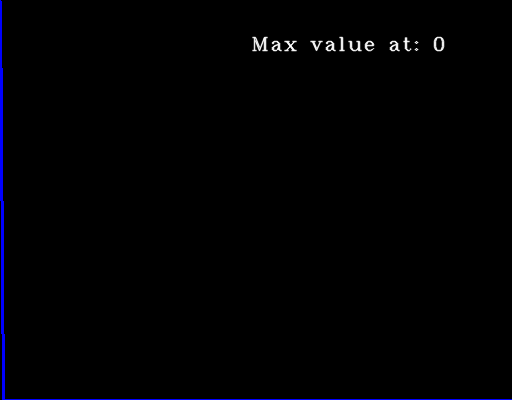
\includegraphics[width=\textwidth]{CV/camera_hls_histogram_1}
		\caption{Hue histogram for test 1}
		\label{fig:hist_test_1}
	\end{subfigure}
	\hfill
	\begin{subfigure}[b]{0.5\textwidth}
		\centering
		
\includegraphics[width=\textwidth]{CV/camera_test_image_1}
		\caption{Image for test 1}
		\label{fig:image_test_1}
	\end{subfigure}
	\caption{Input image and resulting histogram for the 1\textsuperscript{st} test}
	\label{fig:test_1}
\end{figure}

In figure (\ref{fig:hist_test_2}) the hue histogram for the second test can be seen. In this illustration a smaller spike was found with a mean value of 120.
\begin{figure}[H]
	\centering
	\begin{subfigure}[b]{0.48\textwidth}
		\centering
		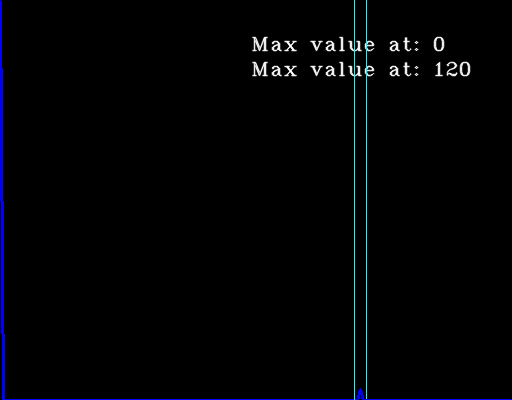
\includegraphics[width=\textwidth]{CV/camera_hls_histogram_2}
		\caption{Hue histogram for test 2}
		\label{fig:hist_test_2}
	\end{subfigure}
	\hfill
	\begin{subfigure}[b]{0.5\textwidth}
		\centering
		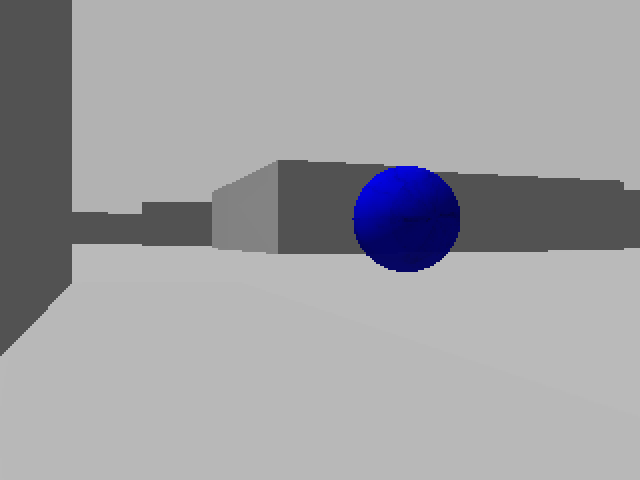
\includegraphics[width=\textwidth]{CV/camera_test_image_2}
		\caption{Image for test 2}
		\label{fig:image_test_2}
	\end{subfigure}
	\caption{Input image and resulting histogram for the 1\textsuperscript{nd} test}
	\label{fig:test_2}
\end{figure}

In figure (\ref{fig:hist_test_3}) the hue histogram for the third test can be seen. In this histogram a larger spike was found at the value of 120.\\
The spike was found at the same value as in test 2, and both spikes correspond to the size of the marble found in the image. Therefore the marbles must have a hue value of 120.
\begin{figure}[H]
	\centering
	\begin{subfigure}[b]{0.48\textwidth}
		\centering
		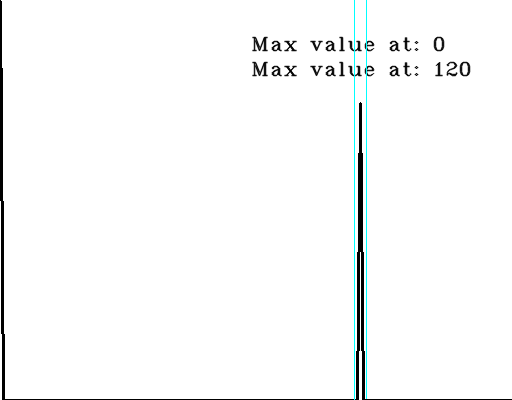
\includegraphics[width=\textwidth]{CV/camera_hls_histogram_5}
		\caption{Hue histogram for test 3}
		\label{fig:hist_test_3}
	\end{subfigure}
	\hfill
	\begin{subfigure}[b]{0.5\textwidth}
		\centering

		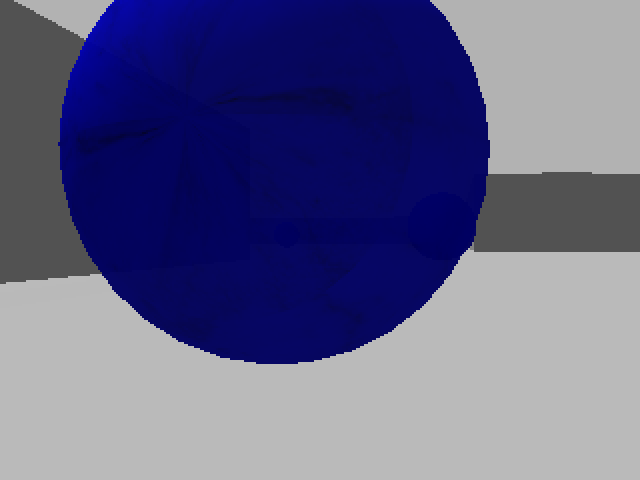
\includegraphics[width=\textwidth]{CV/camera_test_image_5}
		\caption{Image for test 3}
		\label{fig:image_test_3}
	\end{subfigure}
	\caption{Input image and resulting histogram for the 3\textsuperscript{rd} test}
	\label{fig:test_3}
\end{figure}


\subsubsection*{Conclusion}

It can be concluded that the marbles have a hue value around 120. This will be used as a threshold for separating the marbles from the background.

\end{document}